\subsection{Newton's Method}\label{sec:Newton}
A well known numeric method is \ifont{Newton's Method} (also sometimes
referred to as \ifont{Newton-Raphson's Method}), named after Isaac Newton
and Joseph Raphson.  This method is used to find roots, or
$x$-intercepts, of a function.  While we may be able to find the roots
of a polynomial which we can easily factor, we saw in the previous
chapter on {\bf Limits}, that for example the function $e^x + x = 0$
has a solution ($i.e.$ root, or $x$-intercept) at $x \approx
-0.56714$.  By the \ifont{Intermediate Value Theorem} we know that the
function $e^x + x = 0$ does have a solution. We cannot here simply
solve for such a root algebraically, but we can use a numerical method
such as $Newton's$.  Such a process is typically classified as an
$iterative$ method, a name given to a technique which involves
repeating similar steps until the desired accuracy is obtained.   Many
computer $algorithms$ are coded with a for-loop, repeating an
iterative step to converge to a solution.

The idea is to start with an initial value $x_0$ (approximating the
root), and use linear approximation to create values $x_1$, $x_2$, $\cdots$ getting closer and closer to a root. 

The first value $x_1$ corresponds to the intercept of the tangent line
of $f(x_0)$ with the $x$-axis, which is:
\[ x_1 = x_0 -\frac{f(x_0)}{f'(x_0)} \]

\figure[!ht]
$$\includegraphics[width=1.75in]{images/newton_figure_1}$$
\caption{First iteration of Newton's Method. \label{fig:Newton1}} 
\endfigure

We can see in Figure~\ref{fig:Newton1}, that if we compare the point $(x_0,0)$ to
$(x_1,0)$, we would likely come to the conclusion that $(x_1,0)$ is
closer to the actual root of $f(x)$ than our original guess,
$(x_0,0)$.  As will be discussed, the choice of $x_0$ must be done
correctly, and it may occur that $x_1$ does not yield a better
estimate of the root.

Newton's method is simply to repeat this process again and again 
in an effort to obtain a more accurate solution.  Thus at the next step we obtain:

\[ x_2 = x_1 -\frac{f(x_1)}{f'(x_1)} \]

\figure[!ht]
$$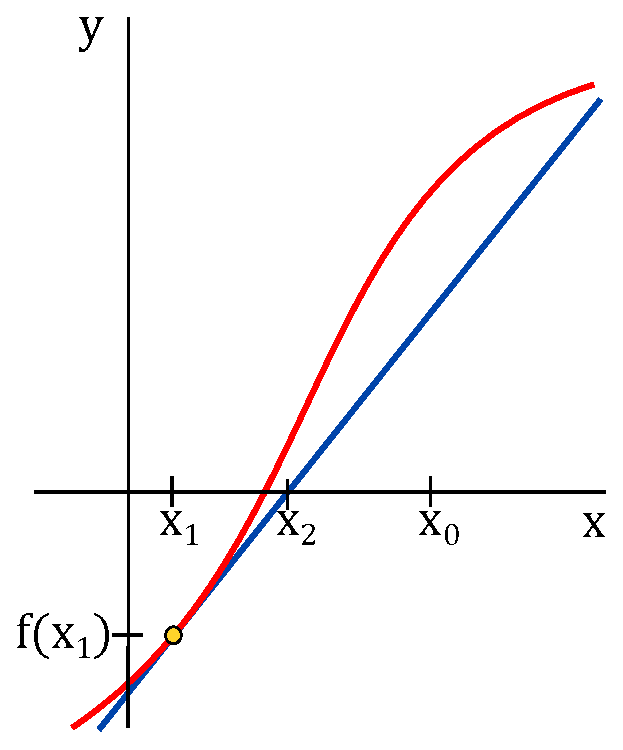
\includegraphics[width=1.75in]{images/newton_figure_2}$$
\caption{Second iteration of Newton's Method. \label{fig:Newton2}}
\endfigure

We can now clearly see how $(x_2,0)$ is a better estimate of the root
of $f(x)$, rather than any of the previous points.  Moving forward, we
will get:
\[ x_3 = x_2 -\frac{f(x_2)}{f'(x_2)} \]
Rest assured, $(x_3,0)$ will be an even better estimate of the root!  We express the general iterative step as:
\[ x_{n+1} = x_n -\frac{f(x_n)}{f'(x_n)} \]

The idea is to iterate these steps to obtain the desired accuracy. Here is an example. 

\begin{example}{Newton method to approximate roots}{newtonroot}
Use Newton's method to approximate the roots of $f(x)=x^3-x+1$.
\end{example}

\begin{solution}
You can try to find solve the equation algebraically to see that this
is a difficult task, and thus it make sense to try a numerical method
such as Newton's.

To find an initial value $x_0$, note that $f(-1)=-5$ and $f(0)=1$,
and by the Intermediate Value Theorem this $f$ has a root between these two values, and we decide to start with $x_0=-1$ (you can try other values to see what happens).

Note that $f'(x)=3x^2-1$, and thus we get
\[ x_{n+1} = x_n -\frac{f(x_n)}{f'(x_n)} = x+n - \frac{x^3_n-x_n+1}{3x^2_n-1} \]
Thus we can produce the following values (try it):
\[ \begin{array}{l}
x_0 = -1 \\
x_1= -1.5000\\
x_2 = -1.347826.. \\
x_3= -1.325200.. \\
x_4 = -1.324718.. \\
x_5 = -1.324717..  \\
x_6 = -1.324717..  \\
\cdots
\end{array} \]
and we can now approximate the root as $-1.324717$.
\end{solution}

As with any numerical method, we need to be aware of the weaknesses of
any technique we are using.

\figure[!ht]
$$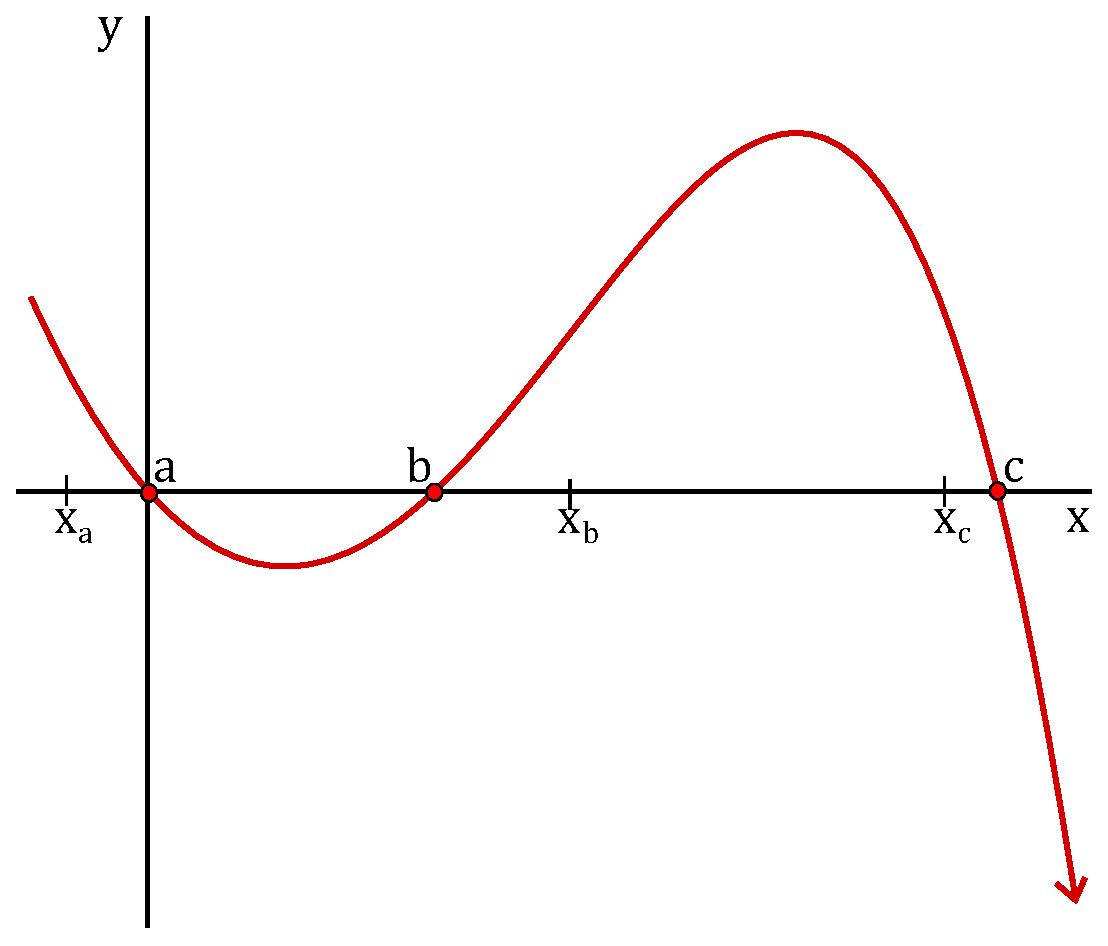
\includegraphics[width=2.5in]{images/newton_figure_4}$$
\caption{Function with three distinct solutions. \label{fig:Newton4}}
\endfigure

%% need an easy example here

If we know our root is somewhere near $a$, we would make our guess
$x_0=a$.  Generally speaking, a good practice is to make our guess as
close to the actual root as possible. In some cases we may have no idea where the root is, so it would be prudent to
perform the algorithm several times on several different initial
guesses and analyze the results. 

For example we can see in Figure~\ref{fig:Newton4} that $f(x)$ in fact has three roots, and depending on our initial
guess, we may get the algorithm to converge to different roots.  If we
did not know where the roots were, we would try the technique several
times.  In one instance, if our initial guess was $x_a$, we'd
likely converge to $(a, 0)$.  Then if we were to choose another
guess, $x_b$, then we'd likely converge to $(b, 0)$.
Eventually, using various initial guesses we'd get one of three roots:
$a$, $b$, or $c$.  Under these circumstances we can
clearly see the effectiveness of this numeric method.

\figure[!ht]
$$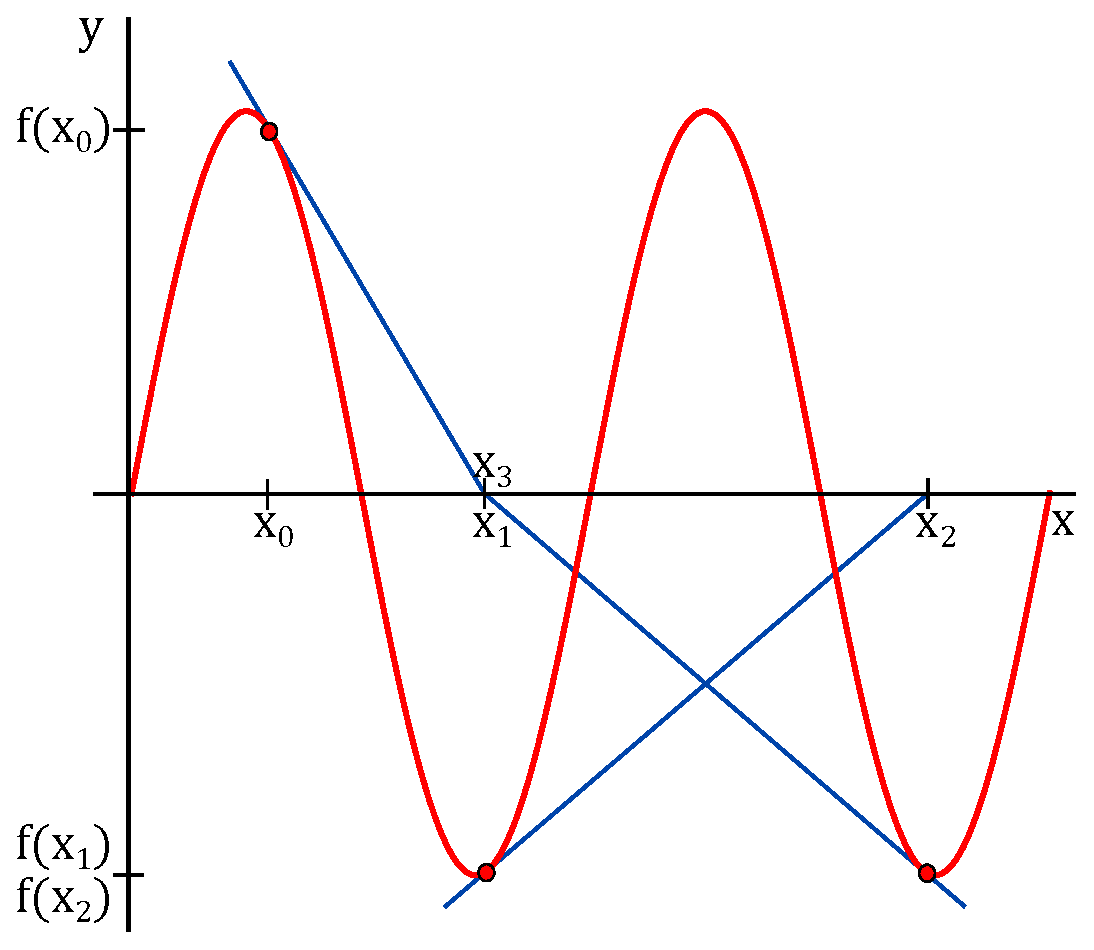
\includegraphics[width=3.5in]{images/newton_figure_3}$$
\caption{Newton's Method applied to $\sin x$. \label{fig:Newton3}}
\endfigure

As another example if we attempt to use $Newton's$ $Method$ on $f(x) =
\sin x$ using $x_0=\pi/2$, then $f'(x_0)=0$ so $x_1$ is undefined and we cannot proceed. 
Even in general $x_{n+1}$ is typically nowhere near $x_n$,
and in general not converging to the root nearest to our initial guess
of $x_0$.  In effect, the algorithm keeps "bouncing around". An example of which is depicted in Figure~\ref{fig:Newton3}. Based on
our initial guess for such a function, the algorithm may or may not
converge to a root, or it may or may not converge to the root {\bf
closest} to the initial guess.  This gives rise to the more common
issue: Selection of the initial guess, $x_0$.

Here is a summary.

{\bf Key Points in using Newton's method to approximate a root of $f(x)$}

\begin{enumerate}
\item Choosing $x_0$ as close as possible to the root we wish to find.
\item A guess for $x_0$ which makes the algorithm ``bounce around'' is considered $unstable$.
\item Even the smallest changes to $x_0$ can have drastic effects: We may converge to another root, 
we may converge very slowly (requiring many more iterations), or we may encounter an unstable point.
\item We may encounter a $stationary$ $point$ if we choose $x_0$ such that $f'(x)=0$ ($i.e.$ at a critical point!) in which case the algorithm fails.
\end{enumerate}

This is all to say that your initial guess for $x_0$ can be extremely
important.


%%%%%%%%%%%%%%%%%%%%%%%%%%%%%%%%%%%%%%%%%%%%%%%
\Opensolutionfile{solutions}[ex]
\section*{Exercises for \ref{sec:Newton}}

\begin{enumialphparenastyle}

%%%%%%%%%%
\begin{ex} 
Use Newton's Method to find all roots of $f(x)=3x^2-9x-11$. (Hint: use Intermediate Value Theorem to choose an appropriate $x_0$)
\begin{sol}
	Notice that $f(-2)=19$, $f(0)=-11$, and $f(5)=19$ and $f$ is a continuous function. By the
	Intermediate Value Theorem there exists a root in $[-2,0]$ and $[0,5]$. Choose $x_0=0$, then $x_4\approx -0.93242$.
	Choose $x_0=5$, then $x_4\approx 3.93242$.
\end{sol}
\end{ex}

%%%%%%%%%%
\begin{ex} 
Consider $f(x)=x^3-x^2+x-1$.
\begin{enumerate}
	\item	Using initial approximation $x_0=2$, find $x_4$.
	\item	What is the exact value of the root of $f$? How does this compare to our approximation $x_4$ in part (a)?
	\item	What would happen if we chose $x_0=0$ as our initial approximation?
\end{enumerate}
\begin{sol}
\begin{enumerate}
	\item	$x_4\approx 1.00022\ldots$
	\item	$x=1$ is the root of $f$. Our approximation in part (a) was correct to 3 decimal places.
	\item	$x_1=1$. The root is found in one iteration of Newton's Method.
\end{enumerate}
\end{sol}
\end{ex}

%%%%%%%%%%
\begin{ex} 
Consider $f(x)=\sin x$. What happens when we choose $x_0=\pi/2$? Explain.
\begin{sol}
	$\cos (\pi/2)=0$, so $x_1$ is undefined.
\end{sol}
\end{ex}

\end{enumialphparenastyle}